\documentclass{article}
\usepackage[utf8]{inputenc}

\title{Informe del parcial 1}
\author{Jackh Emmanuel Narvaez Guerra, Jeisson Arley Alvarez Giraldo, Miguel Angel Alvarez}
\date{April 2021}

\usepackage{natbib}
\usepackage{graphicx}

\begin{document}

\maketitle

\section{Detalles del desarrollo}
nuestra primer idea fue empezar por el desarrollo en el tinkercard idealizando que tendriamos que hacer un circuito en paralelo para poder darle la opcion de encender uno o mas bombillos ya que si fuera en serie si no se prende uno entonces ninguno prende, ya en el transcurso de que fuimos imaginando como seria plantando las ideas de usar transistores y calculando el promedio de las resistencias las ideas empezaron a fluir por si solas, tenemos pensado utiliza matrices y apuntadores para la implementacion del algoritmo en el momento solo es una idea mientras que analizamos bien las situaciones que se puedan presentar en el proceso, tambien creamos el GitHub y nos aseguramos que si pueda ser modificado por cualquiera de nuestros compañeros tuvimos un percanse que uno de los compañeros no tenia el GitHub Destokp y no nos permitia modificar 
-los circuitos en serie no importa si la resistencia la pone por el lado positivo o negativo, se le es indiferente 

\begin{figure}[h!]
\centering
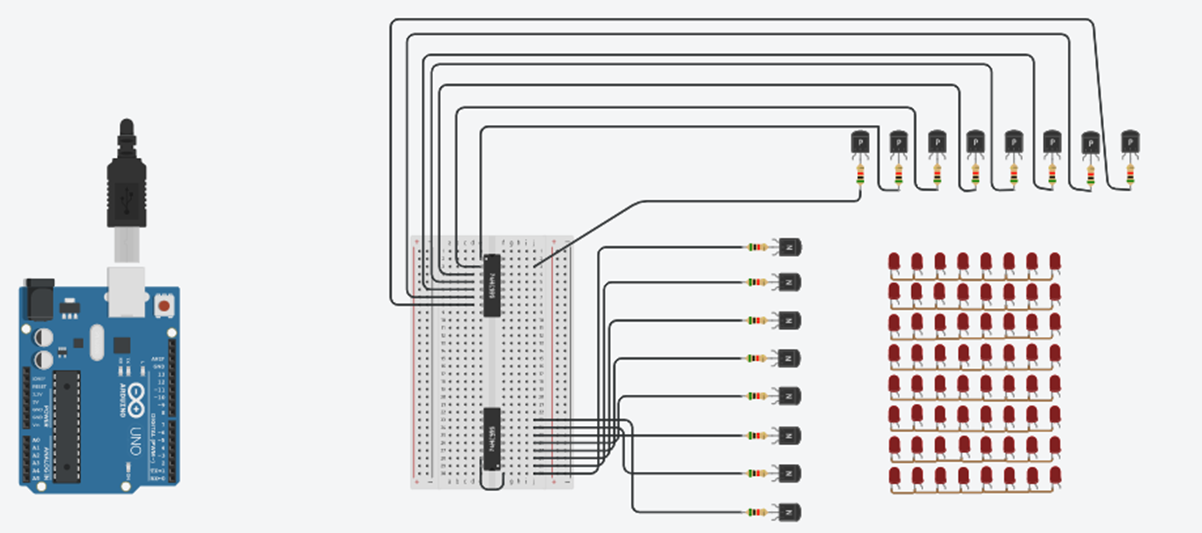
\includegraphics[scale=0.2]{imagen.png}
\caption{primer circuito creado}
\label{fig:universe}
\end{figure}
\section{segundo circuito}
el segundo circuido creado era util pero poco eficiente aparte de eso el nivel de complejidad para poder programarlo era muy alto y el tiempo no nos daria.
\begin{figure}[h!]
\centering
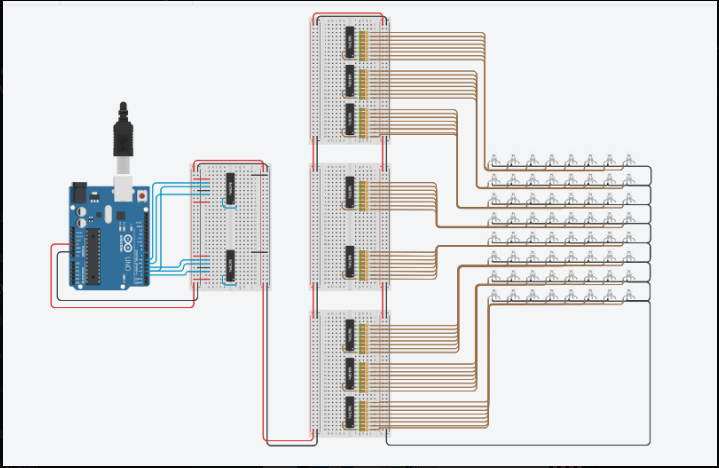
\includegraphics[scale=0.2]{circuito2.PNG}
\caption{segundo circuito creado}
\label{fig:universe}
\end{figure}
\section{tercer circuito}
el tercer circuito creado aparentemente se ve muy bien y funcional ya en este momentos nos dispucimos a estudiar las librearias para poder desarrollar el algoritmo que permita iluminar los leds
\begin{figure}[h!]
\centering
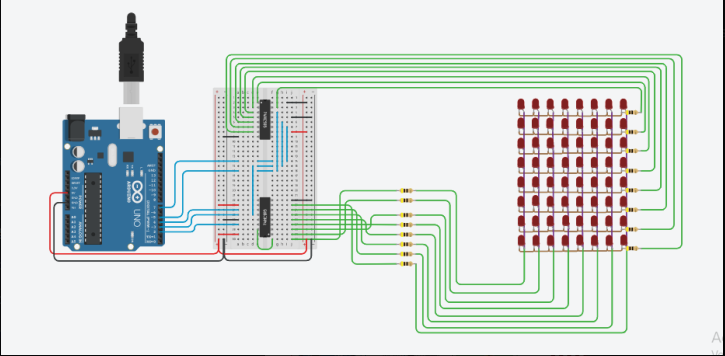
\includegraphics[scale=0.2]{circuito3.PNG}
\caption{tercer circuito creado}
\label{fig:universe}
\end{figure}
\section{problemas del desarrollo}
\begin{itemize}
\item problema1: tuvimos problemas con los transitores, el P funcionaba perfectamente mientras en N tuvimos dudas ya que el P recibe 0 y el N recibe 1, lo cual nos llevo a preguntarnos si se debia a eso.
\item problema2: tuvimos una duda respecto a si se podia usar transistores lo que nos llevo a reiniciar todas las ideas ya propuestas, las resistencias las vamos a empezar a trabajar en 220 ohmio.
\item problema3: tuvimos problemas con el tinkercad, no nos cargaba y el unico compañero que si le cargaba le aparecia un error con el arduino.
\end{itemize}
\begin{figure}[h!]
\centering
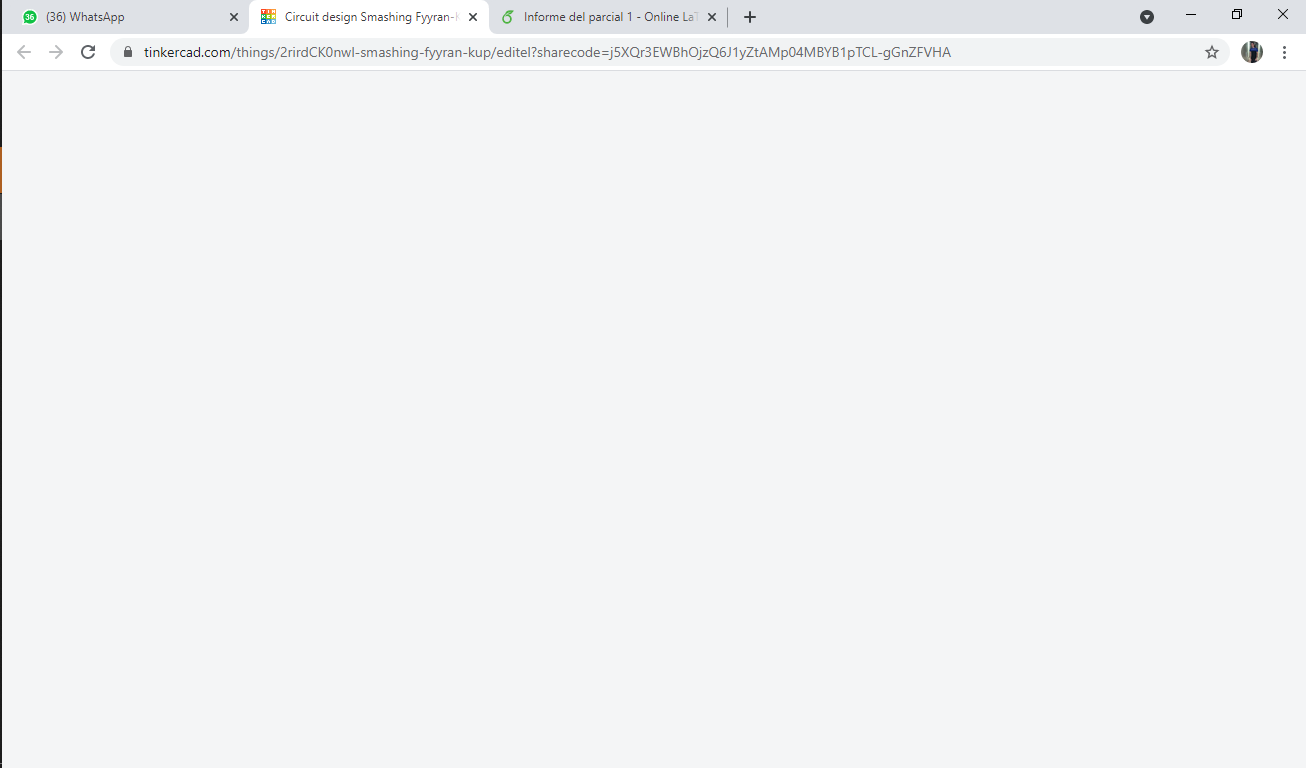
\includegraphics[scale=0.1]{tinkercad.PNG}
\caption{no cargaba la pagina}
\label{fig:universe}
\end{figure}
-lo que le aparecia al compañero que si le cargaba el tinkercad
\begin{figure}[h!]
\centering
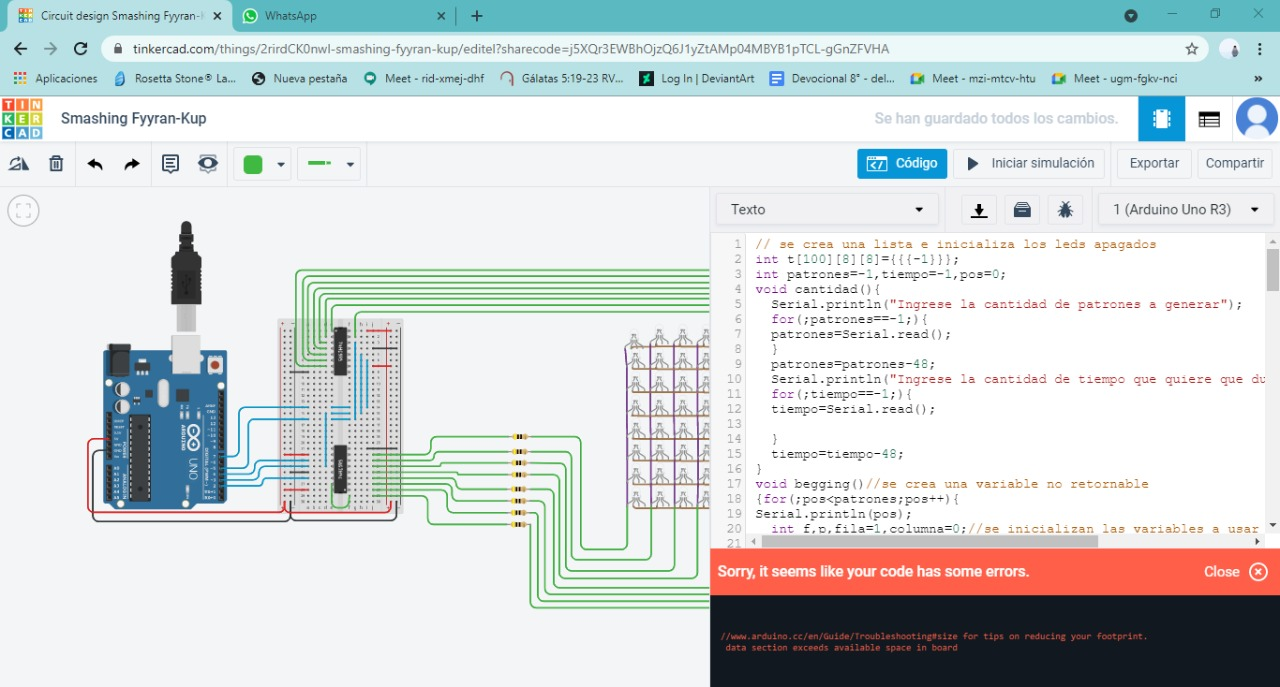
\includegraphics[scale=0.2]{WhatsApp Image 2021-04-21 at 8.39.20 PM.jpeg}
\caption{no cargaba la pagina}
\label{fig:universe}
\end{figure}
\section{circuito final}
\begin{figure}[h!]
\centering
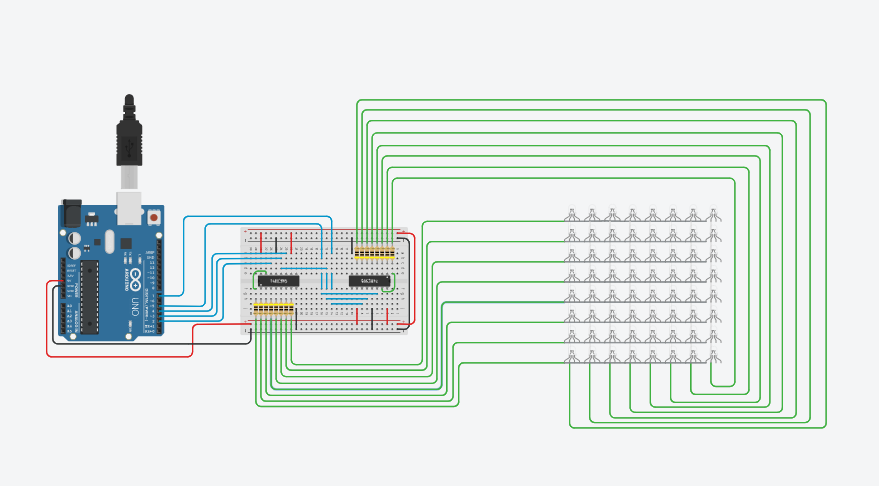
\includegraphics[scale=0.5]{ciruito final.PNG}
\caption{finalizacion del circuito}
\label{fig:universe}
\end{figure}
\section{Conclusion}
este proyecto nos propuso el reto de saber como funciona un circuito y cual es la funcion de cada componente a usar
nos enseño a trabajar en equipo y poder llevar los tiempo para que al hacerle push al repositorio no haya ningun error

\bibliographystyle{plain}
\end{document}
